\section{Stability of the 2-body System using Runge-Kutta and Velovity-Verlet}
\label{sec:stability2bodysystem}

\begin{table}[H]
\centering
\caption{
Initial position and velocity for Earth and Sun in the Sun-Earth-like two-body system. 
F1 refers to the frame of reference at which the Sun is at rest in origo at all times, whilst F2 refers to the frame of reference in which both the Sun and the Earth moves relative to the coordinate axis. 
The mass of the Earth is given in solar masses, that is $M_E = 3.0\times 10^{-6} M_{\odot}$, and the gravitational constant is given is $2.96\cdot 10^{-4} \frac{\textrm{AU}^2}{\textrm{days}^2 \textrm{M}_{\odot}}$ (see \secref{sec:Conversion}).
}
\begin{center}
\begin{tabular}{ | c | c | c |  }
  \hline			
   &  $\v{r}_{initial}$ [AU] & $\v{v}_{initial}$ [AU/day]  
  \\ \hline
  Earth (F1) & $(1.0,0.0,0.0)$ & $(0.0,0.017,0.0)$
  \\ \hline
  Sun (F2) & $(1.0,1.0,1.0)$  & $(0.0,0.0,0.0)$ 
  \\ \hline
  Earth (F2)  & $(2.0,1.0,1.0)$ & $(0.0,0.017,0.0)$
  \\ \hline
\end{tabular}
\end{center}
\label{tab:SunEarthMarsTest}
\end{table}

\begin{figure}[H]
\centering
\begin{minipage}{.5\textwidth}
  \centering
  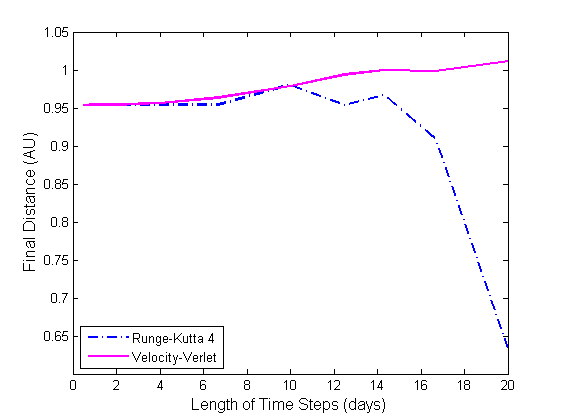
\includegraphics[width=1\linewidth]{Figures/Test_2body_system_earth.png}
\end{minipage}%
\begin{minipage}{.5\textwidth}
  \centering
  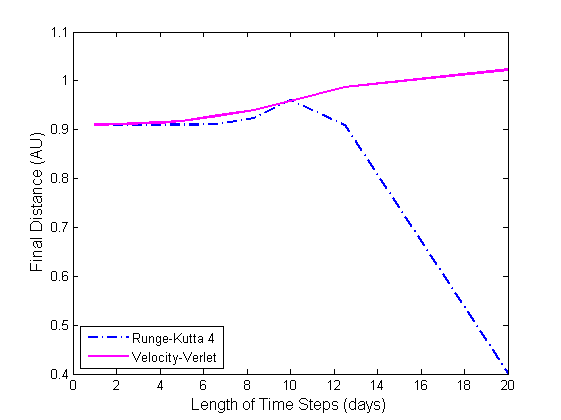
\includegraphics[width=1\linewidth]{Figures/Test_2body_system_earth_sun.png}
\end{minipage}
\caption{
Distance between bodies after 100 years as a function of time step length for the Earth-Sun-like two-body system using both the forth order Runge-Kutta method and the Velocity-Verlet method. 
The leftmost plot do not allow for Sun motion relative to the frame of reference, whilst the rightmost allows for movement of both the Earth and the Sun relative to the frame of reference.
}
\label{fig:SunEarthMarsTest}
\end{figure}

Comment here on, when the methods become stable:
//
around step length of 8 days for RK4 and 4 days for VV ?? \fxnote{fix these lines}

\begin{figure}[H]
\centering
\begin{minipage}{.5\textwidth}
  \centering
  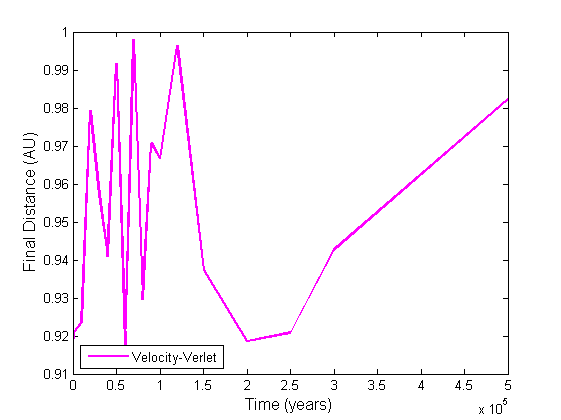
\includegraphics[width=1\linewidth]{Figures/test_distance_time_VV.png}
\end{minipage}%
\begin{minipage}{.5\textwidth}
  \centering
  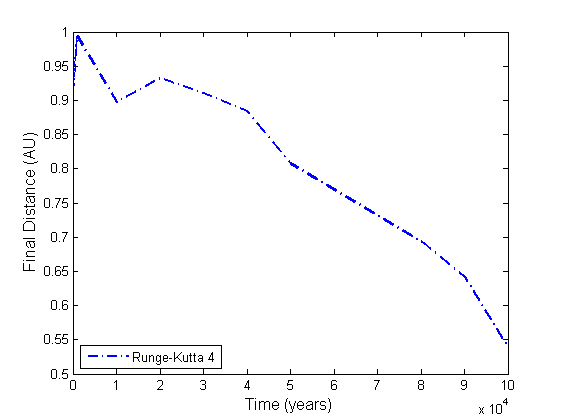
\includegraphics[width=1\linewidth]{Figures/test_distance_time_RK4.png}
\end{minipage}
\caption{
The final distance as a function of time with a time step length of 5 days for both the Velocity-Verlet and Runge-Kutta method with both the Earth and Sun moving relative to the frame of reference.
After $2.5\times 10^4$ years, the Earth continuously moves towards the Sun, in the Runge-Kutta method, whilst the distance between the Earth and Sun still fluctuates between 0.92 AU and 1 AU for the Velocity-Verlet method after $5\times 10^5$ years.  
}
\label{fig:SunEarthMarsTest}
\end{figure}


\begin{table}[H]
\centering
\caption{
Computational time for the fourth order Runge-Kutta method and the Velocity-Verlet method for different time steps during 1 year.
}
\begin{center}
\begin{tabular}{ | c | c | c | }
  \hline			
  \# time steps  & Comp. time RK4 & Comp. time VV  
  \\ \hline
  1 & 6 & 2
  \\ \hline
  10 & 25 & 8
  \\ \hline
  $10^4$ & $8.4\times 10^3$ & $4.6\times 10^3$
  \\ \hline
  $10^6$ & $8.0\times 10^5$ & $3.6\times 10^5$
  \\ \hline
\end{tabular}
\end{center}
\label{tab:SunEarthMarsTest}
\end{table}